%% abtex2-modelo-relatorio-tecnico.tex, v-1.7.1 laurocesar
%% Copyright 2012-2013 by abnTeX2 group at http://abntex2.googlecode.com/ 
%%
%% This work may be distributed and/or modified under the
%% conditions of the LaTeX Project Public License, either version 1.3
%% of this license or (at your option) any later version.
%% The latest version of this license is in
%%   http://www.latex-project.org/lppl.txt
%% and version 1.3 or later is part of all distributions of LaTeX
%% version 2005/12/01 or later.
%%
%% This work has the LPPL maintenance status `maintained'.
%% 
%% The Current Maintainer of this work is the abnTeX2 team, led
%% by Lauro César Araujo. Further information are available on 
%% http://abntex2.googlecode.com/
%%
%% This work consists of the files abntex2-modelo-relatorio-tecnico.tex,
%% abntex2-modelo-include-comandos and abntex2-modelo-references.bib
%%

% ------------------------------------------------------------------------
% ------------------------------------------------------------------------
% abnTeX2: Modelo de Relatório Técnico/Acadêmico em conformidade com 
% ABNT NBR 10719:2011 Informação e documentação - Relatório técnico e/ou
% científico - Apresentação
% ------------------------------------------------------------------------ 
% ------------------------------------------------------------------------

% Alterado por Rodrigo Campiolo para apresentação de relatórios na disciplina
% de Redes de Computadores II do Bacharelado em Ciência da Computação da UTFPR-CM.


\documentclass[
	% -- opções da classe memoir --
	12pt,				% tamanho da fonte
	%openright,			% capítulos começam em pág ímpar (insere página vazia caso preciso)
	oneside,   	        % para impressão em verso e anverso use twoside. Oposto a oneside
	a4paper,			% tamanho do papel. 
	% -- opções da classe abntex2 --
	%chapter=TITLE,		% títulos de capítulos convertidos em letras maiúsculas
	%section=TITLE,		% títulos de seções convertidos em letras maiúsculas
	%subsection=TITLE,	% títulos de subseções convertidos em letras maiúsculas
	%subsubsection=TITLE,% títulos de subsubseções convertidos em letras maiúsculas
	% -- opções do pacote babel --
	english,			% idioma adicional para hifenização
	french,				% idioma adicional para hifenização
	spanish,			% idioma adicional para hifenização
	brazil,				% o último idioma é o principal do documento
	]{pacotes/abntex2}


% ---
% PACOTES
% ---

% ---
% Pacotes fundamentais 
% ---
\usepackage{cmap}				% Mapear caracteres especiais no PDF
\usepackage{lmodern}			% Usa a fonte Latin Modern
\usepackage[T1]{fontenc}		% Selecao de codigos de fonte.
\usepackage[utf8]{inputenc}		% Codificacao do documento (conversão automática dos acentos)
\usepackage{indentfirst}		% Indenta o primeiro parágrafo de cada seção.
\usepackage{color}				% Controle das cores
\usepackage{graphicx}			% Inclusão de gráficos
% ---
\usepackage[utf8]{inputenc}

\usepackage{float}
% ---
% Pacotes adicionais, usados no anexo do modelo de folha de identificação
% ---
\usepackage{multicol}
\usepackage{multirow}
% ---
	
% ---
% Pacotes adicionais, usados apenas no âmbito do Modelo Canônico do abnteX2
% ---
\usepackage{lipsum}				% para geração de dummy text
% ---

% ---
% Pacotes de citações
% ---
\usepackage[brazilian,hyperpageref]{backref}	 % Paginas com as citações na bibl
\usepackage[alf]{pacotes/abntex2cite}	% Citações padrão ABNT
\usepackage{comment}
% --- 
% CONFIGURAÇÕES DE PACOTES
% --- 

% % ---
% % Configurações do pacote backref
% % Usado sem a opção hyperpageref de backref
% \renewcommand{\backrefpagesname}{Citado na(s) página(s):~}
% % Texto padrão antes do número das páginas
% \renewcommand{\backref}{}
% % Define os textos da citação
% \renewcommand*{\backrefalt}[4]{
% 	\ifcase #1 %
% 		Nenhuma citação no texto.%
% 	\or
% 		Citado na página #2.%
% 	\else
% 		Citado #1 vezes nas páginas #2.%
% 	\fi}%
% ---

% ---
% Informações de dados para CAPA e FOLHA DE ROSTO
% ---
\titulo{Escopo de Criação da Empresa UNI-NET}
\autor{Igor Ortega Carmona - RA: 00236524 \\
        Eduardo Fagotti - RA: 00222820 \\
        Kaully Hayashi - RA: 00219066  \\
        Vitor Agostini - RA: 00241431 \\}
\local{Cianorte}
\data{Novembro / 2022}
\instituicao{%
  UNIPAR - CIANORTE
  \par
  Tecnologia em Análise e Desenvolvimento de Sistemas (ADS)
  \par
  Empreendedorismo - Professor e Orientador Dr. Thiago Martins
}
\tipotrabalho{Relatório técnico}
% O preambulo deve conter o tipo do trabalho, o objetivo, 
% o nome da instituição e a área de concentração 
\preambulo{Trabalho feito por alunos e orientado pelo professor Dr. Thiago Martins para a matéria de \textit{Empreendedorismo} grade do curso de \textit{Análise e Desenvolvimento de Sistemas}.}
% ---

% ---
% Configurações de aparência do PDF final

% alterando o aspecto da cor azul
\definecolor{blue}{RGB}{41,5,195}

% informações do PDF
\makeatletter
\hypersetup{
     	%pagebackref=true,
		pdftitle={\@title}, 
		pdfauthor={\@author},
    	pdfsubject={\imprimirpreambulo},
	    pdfcreator={LaTeX with abnTeX2},
		pdfkeywords={abnt}{latex}{abntex}{abntex2}{relatório técnico}, 
		colorlinks=true,       		% false: boxed links; true: colored links
    	linkcolor=blue,          	% color of internal links
    	citecolor=blue,        		% color of links to bibliography
    	filecolor=magenta,      		% color of file links
		urlcolor=blue,
		bookmarksdepth=4
}
\makeatother
% --- 

% --- 
% Espaçamentos entre linhas e parágrafos 
% --- 

% O tamanho do parágrafo é dado por:
\setlength{\parindent}{1.3cm}

% Controle do espaçamento entre um parágrafo e outro:
\setlength{\parskip}{0.2cm}  % tente também \onelineskip

% ---
% compila o indice
% ---
\makeindex
% ---

% Omite a numeração de capítulos
\renewcommand*\thesection{\arabic{section}}



% ----
% Início do documento
% ----
\begin{document}

% Retira espaço extra obsoleto entre as frases.
\frenchspacing 

% ----------------------------------------------------------
% ELEMENTOS PRÉ-TEXTUAIS
% ----------------------------------------------------------
% \pretextual

% ---
% Capa
% ---
%\imprimircapa
% ---

% ---
% Folha de rosto
% (o * indica que haverá a ficha bibliográfica)
% ---
\imprimirfolhaderosto
% ---


% ---
% RESUMO
% ---

% resumo na língua vernácula (obrigatório)
\begin{resumo}
 
 Um software capaz de conectar alunos, professores e empresas em um só lugar promovendo assim, uma base para sustentar a ideia de estágios para universitários e aumentar a rede de network.

 \vspace{\onelineskip}
    
 \noindent
 \textbf{Palavras-chave}: uni-net, empresa, empreendedorismo.
\end{resumo}
% ---

% ---
% inserir lista de ilustrações
% ---
%\pdfbookmark[0]{\listfigurename}{lof}
%\listoffigures*
%\cleardoublepage
% ---

% ---
% inserir lista de tabelas
% ---
%\pdfbookmark[0]{\listtablename}{lot}
%\listoftables*
%\cleardoublepage
% ---

% ---
% inserir lista de abreviaturas e siglas
% ---
%\begin{siglas}
%  \item[IP] Internet Protocol
%  \item[TCP] Transmission Control Protocol
%  \item[UDP] User Datagram Protocol
%\end{siglas}
% ---

% ---
% inserir o sumario
% ---
\pdfbookmark[0]{\contentsname}{toc}
\tableofcontents*
\cleardoublepage
% ---

% ----------------------------------------------------------
% ELEMENTOS TEXTUAIS
% ----------------------------------------------------------

%------------------------------------------------------------------------%
%% PARA FAZER CITAÇÕES
  %  \cite{kernel/Linux}.
%------------------------------------------------------------------------%


%------------------------------------------------------------------------%
%%LISTAGEM DE ITENS

%\begin{itemize}
%    \item \textbf{Virtual Box 6.1:} TEXTO
%\end{itemize}
%\begin{itemize}
%    \item \textbf{Distribuição Linux GNU/Debian 11.4:} TEXTO
%\end{itemize}
%\begin{itemize}
%    \item \textbf{kernel Linux 5.19.2:} TEXTO
%\end{itemize}
%------------------------------------------------------------------------%


%-------------------------------------------------------------------------%
  %% COLOCAR SITES
  
 % \url{https://www.debian.org/download}.
%-------------------------------------------------------------------------%
 
 
%-------------------------------------------------------------------------%    
%%%% COLOCAR FIGURAS %%%%

 %   \begin{figure}[H]
  %\centering
  %\includegraphics[scale=0.8]{figuras/vm.png}
  %\caption{Configurações inicias da máquina}
  %\label{fig:partições}
%\end{figure}
%------------------------------------------------------------------------%

\textual

\makeatletter
\renewcommand{\chapter}{\@gobbletwo}
\makeatother

\section{\textbf{Dados dos Empreendedores, Experiência Profissional e Atribuições}}
\label{sec:pessoas-empreen}

\textbf{Igor Carmona, 22 anos –}\textit{Desenvolvedor back-end}: Coordenador de equipe back-end, contato direto com o cliente e atua na resolução de problemas internos ao software.

\textbf{Kaully Hayashi, 19 anos – }\textit{Diretora da empresa}: Controle de procedimentos operacionais, administração geral, reunião diária com fornecedores e desenvolvedores.

\textbf{Eduardo Fagotti, 21 anos –}\textit{Desenvolvedor front-end}: Coordenador de equipe front-end, responsável pela criação de layouts de acordo com o figma do design.

\textbf{Vitor Agostini, 22 anos – }\textit{Auxiliar administrativo/Financeiro}: Responsável pelos tributos da empresa, coordenador de equipe financeira, arquivamento de processos, contas a pagar e atividades internas relativas.


\section{\textbf{Dados do Empreendimento}}
\label{sec:dados-empreen}

\textbf{Nome da empresa}: UNI-NET.

\textbf{Razão Social}: Uni-Net Desenvolvimento Educacional LTDA.

\textbf{CNPJ}: Em processo.


\section{\textbf{Missão, Valores e Visão da Empresa}}
\label{sec:missão}

\subsection{\textbf{Missão da Empresa}}
\label{subsec:missão}

Sistema capaz de conectar: alunos, professores e empresas de forma homogênea.

\subsection{\textbf{Visão da Empresa}}
\label{subsec:visão}

Aumento de comunicação entre os alunos e empresas criando uma maior rede de network.

\subsection{\textbf{Valores da Empresa}}
\label{subsec:valores}

Igualdade, solidariedade, empregabilidade.

\section{\textbf{Setores de Atividades}}
\label{sec:setores}

Área educacional (B2B) e serviço ao governo (B2G).

\section{\textbf{Forma Jurídica}}
\label{sec:juridica}

Sociedade Comercial por quotas de responsabilidades (LTDA).

\section{\textbf{Enquadramento Tributário}}
\label{sec:enquadramento}

Empresa de pequeno porte (EPP).

\section{\textbf{Capital Social}}
\label{sec:capital}

A UNI-NET tem capital social de R\$50.000,00 reais.

\section{\textbf{Fonte de Recursos}}
\label{sec:recursos}

Capital próprio e empresas parceiras voltadas a área educacional.

\section{\textbf{Estudo dos Clientes}}
\label{sec:estudo}

A maior “dor” que encontramos seria na busca de funcionários capacitados para as empresas, empregabilidade aos universitários e a diminuição de desistências dos cursos pela falta de entendimento de matérias e afins, já que nosso aplicativo conta com sessões onde os universitários podem trocar conhecimentos e sanar dúvidas juntamente aos professores.

Nosso diferencial é o \textbf{“uni godfather” (UGF)}, do português: \textbf{Padrinho da universidade}, onde um veterano apadrinha dois ou mais calouros dando suporte em matérias pelas quais já passou.


\section{\textbf{Cliente Ideal}}
\label{sec:cliente-ideal}

Universidades que buscam implementar um sistema de conexão entre os próprios alunos e empresas, diminuindo desistências de curso e aumentando a empregabilidade local por um valor acessível.

\section{\textbf{Estudo de Concorrentes e Fornecedores}}
\label{sec:estudos-empresas}

\subsection{\textbf{Estudo Concorrentes}}
\label{subsec:concorrentes}

\begin{figure}[H]
  \centering
  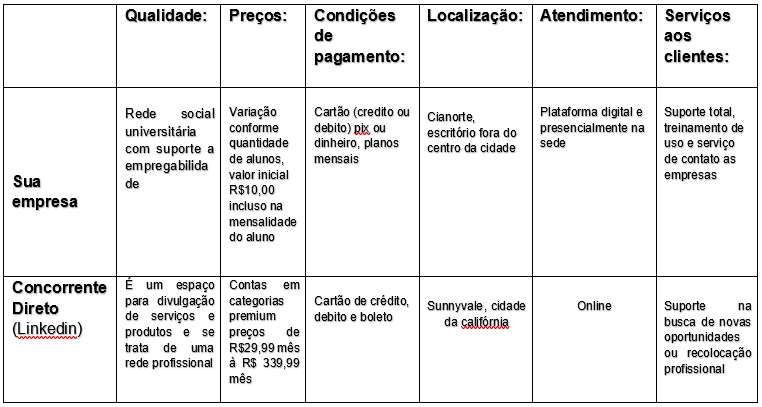
\includegraphics[scale=0.8]{Figuras/fig-concorrentes.png}
  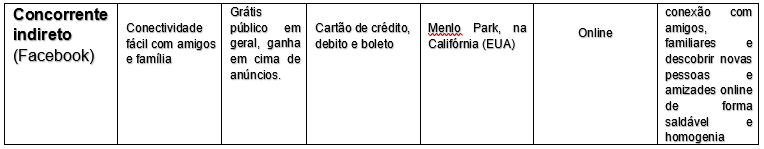
\includegraphics[scale=0.8]{Figuras/fig-concorrente2.png}
  \caption{Análise da UNI-NET junto as empresas concorrentes diretas e indiretas.\cite{imagem1}}
  \label{fig:concorrentes}
\end{figure}

\subsection{\textbf{Estudo Fornecedores}}
\label{subsec:fornecedores}

\begin{figure}[H]
  \centering
  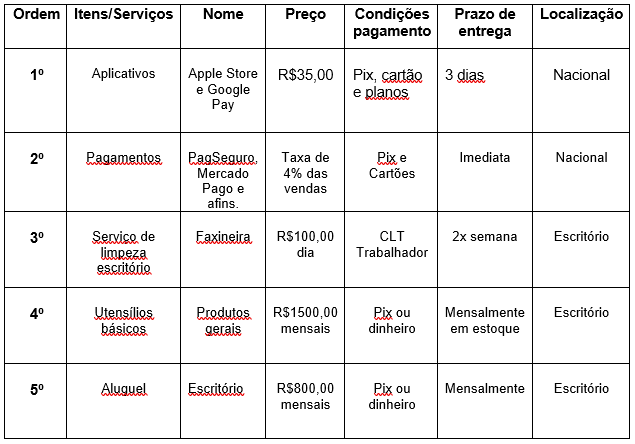
\includegraphics[scale=0.9]{Figuras/fig-fornecedores.png}
  \caption{Análise de fornecedores e dos itens.\cite{imagem2}}
  \label{fig:fornecedores}
\end{figure}

\section{\textbf{Plano de Marketing}}
\label{sec:plano}

\subsection{\textbf{Descrição dos Principais Produtos e Serviços}}
\label{subsec:principais-produtos}

Nossa \textbf{marca} está comprometida em entregar o melhor software com base no feedback e a necessidade do cliente, escolhemos também, cores mais frias como o azul e branco pois passa uma sensação de um ambiente agradável visando sempre a \textbf{qualidade} do produto final. 

\begin{figure}[H]
  \centering
  
\includegraphics[scale=0.8]{Figuras/fig-logo.png}
  \caption{Logo da UNI-NET.}
  \label{fig:logo-uni}
\end{figure}

Após a finalização da venda a UNI-NET irá enviar uma carta para o cliente agradecendo-o pela compra, no caso, seria a nossa \textbf{embalagem} do produto além do design dos layouts criados pela equipe de front-end. 

\begin{figure}[H]
  \centering
  \includegraphics[scale=0.6]{Figuras/fig-cartão.png}
  \caption{Cartão de apresentação da UNI-NET}
  \label{fig:cartão}
\end{figure}

A UNI-NET possui \textbf{serviço} em vídeo aulas de tutorias de como manipular o software para melhor entendimento dos clientes, suporte direto para dúvidas e contato direto para empresas para inclusão no aplicativo. Ofertamos também ao cliente, uma \textbf{garantia} de 3 meses de uso sem mensalidade.

\section{\textbf{Estratégias de Preço}}
\label{sec:preço-estratégia}

Pensando em relação aos alunos e ao cliente, indicamos os clientes a colocar o preço do nosso produto incluso na mensalidade do aluno, antes do estudante fazer a matricula na universidade ele é advertido de um valor adicional de R\$30,00 incluso na sua fatura tendo ele a opção de aceitar ou não o nosso software. 

\section{\textbf{Descontos}}
\label{sec:descontos}

O cliente também tem desconto chamando outros clientes. Por exemplo, chama 3 amigos e ganha um desconto de 5\%. A cada 1000 alunos tem desconto de 5\% e 2000 alunos 10\% e 3000 alunos tem 15\% de desconto.

\section{\textbf{Formas de Pagamento}}
\label{sec:formas-pagamento}

Através de dinheiro, pix, cartão de crédito ou debito, devido a ser uma empresa de desenvolvimento de software, os planos mensais seria a renda mais procurada.

\section{\textbf{Estratégias Promocionais}}
\label{sec:formas-pagamento}

Parcerias locais divulgariam seus produtos com o QRCODE de nossa empresa o que criaria pessoas interessadas em nosso produto ou para fixar a logo e a identidade visual para que ao comentarmos sobre já venha a mente UNI-NET. Tendo em vista a divulgação o público-alvo: Estudantes.

\section{\textbf{Localização do Negócio}}
\label{sec:local}

Por se tratar de uma empresa online, os colaboradores poderão trabalhar em suas casas recebendo total suporte financeiro.

\section{\textbf{Pitch}}
\label{sec:pitch}

Está sendo disponibilizado o link para visualização do vídeo de Pitch da empresa UNI-NET pelo \textit{YouTube}.

\begin{itemize}
    \item \textbf{Link YouTube:} \url{https://youtu.be/359c_LrHgYo}.
\end{itemize}

\section{\textbf{Plano Operacional}}
\label{sec:plano-operacional}

\subsection{\textbf{Custos Gerais}}
\label{subsec:custos-gerais}

\subsubsection{\textbf{Custos fixos}}
\begin{figure}[H]
  \centering
  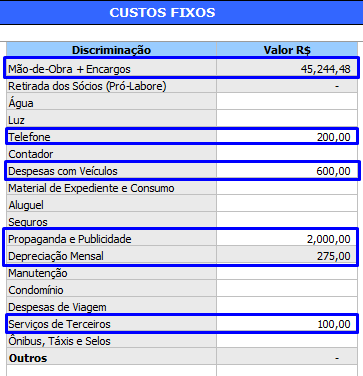
\includegraphics[scale=1.0]{Figuras/custos fixos.png}
  \caption{Custos fixos de acordo com tabela de Plano de Negócio da \textit{SEBRAE}}
  \label{fig:custos-fixos}
\end{figure}

\subsubsection{\textbf{Custo de mão-de-obra}}
\begin{figure}[H]
  \centering
  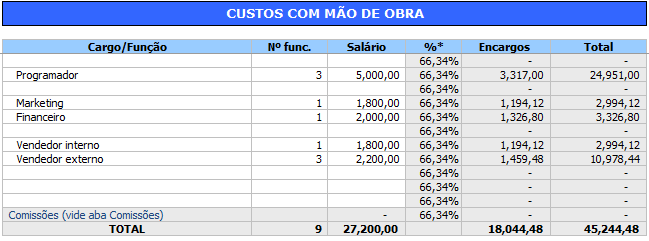
\includegraphics[scale=1.0]{Figuras/Custo mao de obra.png}
  \caption{Custos de mão-de-obra de acordo com tabela de Plano de Negócio da \textit{SEBRAE}}
  \label{fig:custos-obra}
\end{figure}

\subsubsection{\textbf{Investimento fixo}}
\begin{figure}[H]
  \centering
  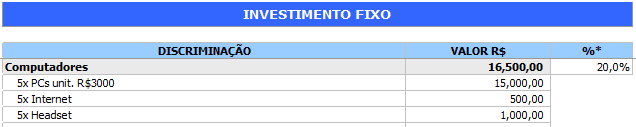
\includegraphics[scale=1.0]{Figuras/investimento fixo.png}
  \caption{Investimento fixo de acordo com tabela de Plano de Negócio da \textit{SEBRAE}}
  \label{fig:investimento-fixo}
\end{figure}

\subsubsection{\textbf{Faturamento mensal}}
\begin{figure}[H]
  \centering
  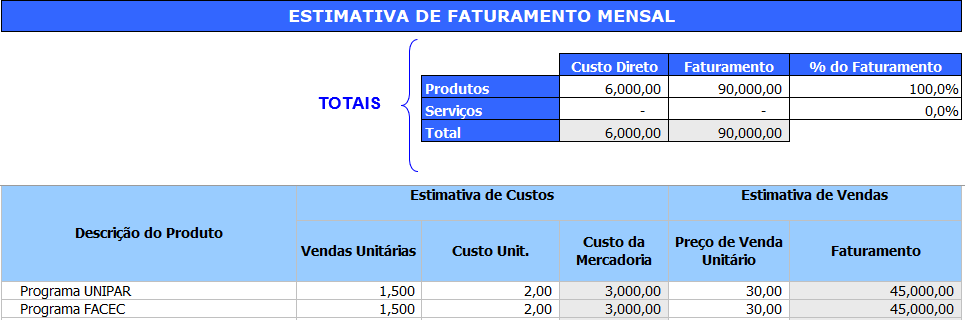
\includegraphics[scale=0.7]{Figuras/faturamento.png}
  \caption{Faturamento mensal de acordo com tabela de Plano de Negócio da \textit{SEBRAE}}
  \label{fig:faturamento}
\end{figure}

\subsection{\textbf{Indicadores financeiros}}
\label{subsec:indicadores}

\begin{figure}[H]
  \centering
  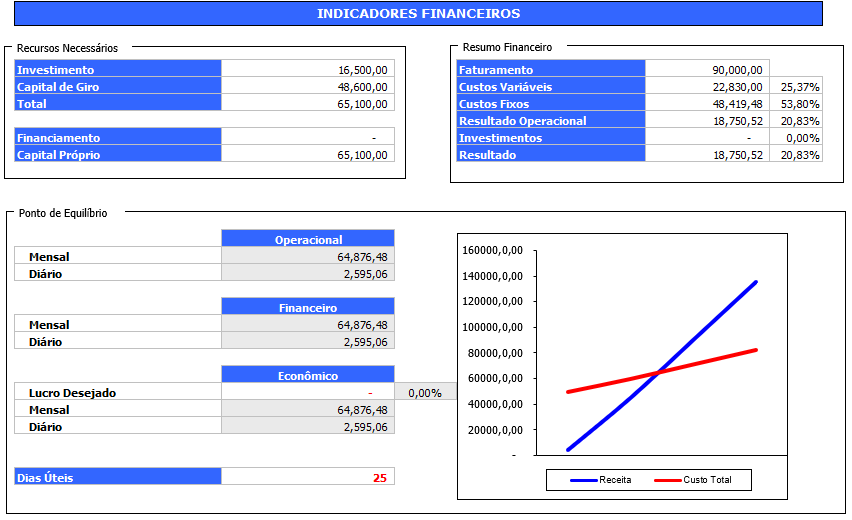
\includegraphics[scale=0.8]{Figuras/indicadores.png}
  \caption{Indicadores financeiros de acordo com tabela de Plano de Negócio da \textit{SEBRAE}}
  \label{fig:indicadores}
\end{figure}

\subsection{\textbf{Local de trabalho}}
\label{subsec:local-trabalho}

Os colaboradores da nossa empresa trabalharão de forma remota, apenas os nossos vendedores externos não terão atividades remotas e atuarão nas ruas e nas faculdades em geral aplicando divulgações e palestras de nosso produto.

\subsection{\textbf{Cenários de Possíveis Eventos}}
\label{subsec:cenários}

\begin{itemize}
    \item \textbf{PLANO A}: 
        \textit{Ter 20\% das universidades do paraná como nossos clientes.}
    \item \textbf{PLANO B}: 
        \textit{Conseguir 3 universidades como clientes na cidade natal da empresa.}
    \item \textbf{PLANO C}: 
        \textit{Ficar com pelo menos 1 universidade por uma mensalidade mais alta.}
\end{itemize}

\subsection{\textbf{Descrição de Força, Fraqueza, Oportunidade e Ameaça}}
\label{subsec:fofa}

\begin{itemize}
    \item \textbf{FORÇA}: 
        \textit{Programadores especializados, sem custo de matéria-prima, mensalidade baixa, fácil acesso, redução nos custos de operação.}
    \item \textbf{FRAQUEZA}: 
        \textit{Vendedor despreparado, sem loja física, acesso a empresa somente pela internet.}
    \item \textbf{OPORTUNIDADE}: 
        \textit{Possibilidade de clientes no exterior, possibilidade de alcançar muitos clientes, alcançar não somente faculdades mas escolas públicas de ensino médio.}
    \item \textbf{AMEAÇA}: 
        \textit{Linkedin, pois atua quase no mesmo ramo que a UNI-NET e o Facebook, pois tem uma grande interatividade com os usuários.}
\end{itemize}

\section{\textbf{CONCLUSÃO: Afinal, esse projeto é viável ou não manter?}}
\label{sec:conclusao}

Contudo, a resposta é sim! Pois em todas os planos A,B e C ainda conseguimos obter lucro com o negócio e as oportunidades que possam vir a surgir estão a nosso favor. 

\newpage
% ----------------------------------------------------------
% ELEMENTOS PÓS-TEXTUAIS
% ----------------------------------------------------------
\postextual
% ----------------------------------------------------------
% Referências bibliográficas
% ----------------------------------------------------------
\renewcommand{\bibsection}{%
\section{\bibname}
\bibmark
%\ifnobibintoc\else
%\phantomsection
%\addcontentsline{toc}{section}{\bibname}
%\fi
\prebibhook}

\bibliography{abntex2-modelo-references}

% ----------------------------------------------------------
% Apêndices
% ----------------------------------------------------------

% ---
% Inicia os apêndices
% ---
% \begin{apendicesenv}

% % ----------------------------------------------------------
% \section*{Apêndice A - Nome do Apêndice}
% \addcontentsline{toc}{section}{Apêndice A - Nome do Apêndice}
% % ----------------------------------------------------------

% \end{apendicesenv}
% % ---


% ----------------------------------------------------------
% Anexos
% ----------------------------------------------------------

% % ---
% % Inicia os anexos
% % ---
% \begin{anexosenv}

% % ---
% \section*{Anexo A - Nome do Anexo}
% \addcontentsline{toc}{section}{Anexo A - Nome do Anexo}
% % ---
% \end{anexosenv}


\end{document}
